\documentclass[11pt]{article}
\usepackage{ACL}
\usepackage{times}
\usepackage{url}
\usepackage{latexsym}
\usepackage{enumitem}
\usepackage{subfigure}
\usepackage{graphicx}
%%%%% NEW MATH DEFINITIONS %%%%%

\usepackage{amsmath,amsfonts,bm}

% Mark sections of captions for referring to divisions of figures
\newcommand{\figleft}{{\em (Left)}}
\newcommand{\figcenter}{{\em (Center)}}
\newcommand{\figright}{{\em (Right)}}
\newcommand{\figtop}{{\em (Top)}}
\newcommand{\figbottom}{{\em (Bottom)}}
\newcommand{\captiona}{{\em (a)}}
\newcommand{\captionb}{{\em (b)}}
\newcommand{\captionc}{{\em (c)}}
\newcommand{\captiond}{{\em (d)}}

% Highlight a newly defined term
\newcommand{\newterm}[1]{{\bf #1}}


% Figure reference, lower-case.
\def\figref#1{figure~\ref{#1}}
% Figure reference, capital. For start of sentence
\def\Figref#1{Figure~\ref{#1}}
\def\twofigref#1#2{figures \ref{#1} and \ref{#2}}
\def\quadfigref#1#2#3#4{figures \ref{#1}, \ref{#2}, \ref{#3} and \ref{#4}}
% Section reference, lower-case.
\def\secref#1{section~\ref{#1}}
% Section reference, capital.
\def\Secref#1{Section~\ref{#1}}
% Reference to two sections.
\def\twosecrefs#1#2{sections \ref{#1} and \ref{#2}}
% Reference to three sections.
\def\secrefs#1#2#3{sections \ref{#1}, \ref{#2} and \ref{#3}}
% Reference to an equation, lower-case.
\def\eqref#1{equation~\ref{#1}}
% Reference to an equation, upper case
\def\Eqref#1{Equation~\ref{#1}}
% A raw reference to an equation---avoid using if possible
\def\plaineqref#1{\ref{#1}}
% Reference to a chapter, lower-case.
\def\chapref#1{chapter~\ref{#1}}
% Reference to an equation, upper case.
\def\Chapref#1{Chapter~\ref{#1}}
% Reference to a range of chapters
\def\rangechapref#1#2{chapters\ref{#1}--\ref{#2}}
% Reference to an algorithm, lower-case.
\def\algref#1{algorithm~\ref{#1}}
% Reference to an algorithm, upper case.
\def\Algref#1{Algorithm~\ref{#1}}
\def\twoalgref#1#2{algorithms \ref{#1} and \ref{#2}}
\def\Twoalgref#1#2{Algorithms \ref{#1} and \ref{#2}}
% Reference to a part, lower case
\def\partref#1{part~\ref{#1}}
% Reference to a part, upper case
\def\Partref#1{Part~\ref{#1}}
\def\twopartref#1#2{parts \ref{#1} and \ref{#2}}

\def\ceil#1{\lceil #1 \rceil}
\def\floor#1{\lfloor #1 \rfloor}
\def\1{\bm{1}}
\newcommand{\train}{\mathcal{D}}
\newcommand{\valid}{\mathcal{D_{\mathrm{valid}}}}
\newcommand{\test}{\mathcal{D_{\mathrm{test}}}}

\def\eps{{\epsilon}}


% Random variables
\def\reta{{\textnormal{$\eta$}}}
\def\ra{{\textnormal{a}}}
\def\rb{{\textnormal{b}}}
\def\rc{{\textnormal{c}}}
\def\rd{{\textnormal{d}}}
\def\re{{\textnormal{e}}}
\def\rf{{\textnormal{f}}}
\def\rg{{\textnormal{g}}}
\def\rh{{\textnormal{h}}}
\def\ri{{\textnormal{i}}}
\def\rj{{\textnormal{j}}}
\def\rk{{\textnormal{k}}}
\def\rl{{\textnormal{l}}}
% rm is already a command, just don't name any random variables m
\def\rn{{\textnormal{n}}}
\def\ro{{\textnormal{o}}}
\def\rp{{\textnormal{p}}}
\def\rq{{\textnormal{q}}}
\def\rr{{\textnormal{r}}}
\def\rs{{\textnormal{s}}}
\def\rt{{\textnormal{t}}}
\def\ru{{\textnormal{u}}}
\def\rv{{\textnormal{v}}}
\def\rw{{\textnormal{w}}}
\def\rx{{\textnormal{x}}}
\def\ry{{\textnormal{y}}}
\def\rz{{\textnormal{z}}}

% Random vectors
\def\rvepsilon{{\mathbf{\epsilon}}}
\def\rvtheta{{\mathbf{\theta}}}
\def\rva{{\mathbf{a}}}
\def\rvb{{\mathbf{b}}}
\def\rvc{{\mathbf{c}}}
\def\rvd{{\mathbf{d}}}
\def\rve{{\mathbf{e}}}
\def\rvf{{\mathbf{f}}}
\def\rvg{{\mathbf{g}}}
\def\rvh{{\mathbf{h}}}
\def\rvu{{\mathbf{i}}}
\def\rvj{{\mathbf{j}}}
\def\rvk{{\mathbf{k}}}
\def\rvl{{\mathbf{l}}}
\def\rvm{{\mathbf{m}}}
\def\rvn{{\mathbf{n}}}
\def\rvo{{\mathbf{o}}}
\def\rvp{{\mathbf{p}}}
\def\rvq{{\mathbf{q}}}
\def\rvr{{\mathbf{r}}}
\def\rvs{{\mathbf{s}}}
\def\rvt{{\mathbf{t}}}
\def\rvu{{\mathbf{u}}}
\def\rvv{{\mathbf{v}}}
\def\rvw{{\mathbf{w}}}
\def\rvx{{\mathbf{x}}}
\def\rvy{{\mathbf{y}}}
\def\rvz{{\mathbf{z}}}

% Elements of random vectors
\def\erva{{\textnormal{a}}}
\def\ervb{{\textnormal{b}}}
\def\ervc{{\textnormal{c}}}
\def\ervd{{\textnormal{d}}}
\def\erve{{\textnormal{e}}}
\def\ervf{{\textnormal{f}}}
\def\ervg{{\textnormal{g}}}
\def\ervh{{\textnormal{h}}}
\def\ervi{{\textnormal{i}}}
\def\ervj{{\textnormal{j}}}
\def\ervk{{\textnormal{k}}}
\def\ervl{{\textnormal{l}}}
\def\ervm{{\textnormal{m}}}
\def\ervn{{\textnormal{n}}}
\def\ervo{{\textnormal{o}}}
\def\ervp{{\textnormal{p}}}
\def\ervq{{\textnormal{q}}}
\def\ervr{{\textnormal{r}}}
\def\ervs{{\textnormal{s}}}
\def\ervt{{\textnormal{t}}}
\def\ervu{{\textnormal{u}}}
\def\ervv{{\textnormal{v}}}
\def\ervw{{\textnormal{w}}}
\def\ervx{{\textnormal{x}}}
\def\ervy{{\textnormal{y}}}
\def\ervz{{\textnormal{z}}}

% Random matrices
\def\rmA{{\mathbf{A}}}
\def\rmB{{\mathbf{B}}}
\def\rmC{{\mathbf{C}}}
\def\rmD{{\mathbf{D}}}
\def\rmE{{\mathbf{E}}}
\def\rmF{{\mathbf{F}}}
\def\rmG{{\mathbf{G}}}
\def\rmH{{\mathbf{H}}}
\def\rmI{{\mathbf{I}}}
\def\rmJ{{\mathbf{J}}}
\def\rmK{{\mathbf{K}}}
\def\rmL{{\mathbf{L}}}
\def\rmM{{\mathbf{M}}}
\def\rmN{{\mathbf{N}}}
\def\rmO{{\mathbf{O}}}
\def\rmP{{\mathbf{P}}}
\def\rmQ{{\mathbf{Q}}}
\def\rmR{{\mathbf{R}}}
\def\rmS{{\mathbf{S}}}
\def\rmT{{\mathbf{T}}}
\def\rmU{{\mathbf{U}}}
\def\rmV{{\mathbf{V}}}
\def\rmW{{\mathbf{W}}}
\def\rmX{{\mathbf{X}}}
\def\rmY{{\mathbf{Y}}}
\def\rmZ{{\mathbf{Z}}}

% Elements of random matrices
\def\ermA{{\textnormal{A}}}
\def\ermB{{\textnormal{B}}}
\def\ermC{{\textnormal{C}}}
\def\ermD{{\textnormal{D}}}
\def\ermE{{\textnormal{E}}}
\def\ermF{{\textnormal{F}}}
\def\ermG{{\textnormal{G}}}
\def\ermH{{\textnormal{H}}}
\def\ermI{{\textnormal{I}}}
\def\ermJ{{\textnormal{J}}}
\def\ermK{{\textnormal{K}}}
\def\ermL{{\textnormal{L}}}
\def\ermM{{\textnormal{M}}}
\def\ermN{{\textnormal{N}}}
\def\ermO{{\textnormal{O}}}
\def\ermP{{\textnormal{P}}}
\def\ermQ{{\textnormal{Q}}}
\def\ermR{{\textnormal{R}}}
\def\ermS{{\textnormal{S}}}
\def\ermT{{\textnormal{T}}}
\def\ermU{{\textnormal{U}}}
\def\ermV{{\textnormal{V}}}
\def\ermW{{\textnormal{W}}}
\def\ermX{{\textnormal{X}}}
\def\ermY{{\textnormal{Y}}}
\def\ermZ{{\textnormal{Z}}}

% Vectors
\def\vzero{{\bm{0}}}
\def\vone{{\bm{1}}}
\def\vmu{{\bm{\mu}}}
\def\vtheta{{\bm{\theta}}}
\def\va{{\bm{a}}}
\def\vb{{\bm{b}}}
\def\vc{{\bm{c}}}
\def\vd{{\bm{d}}}
\def\ve{{\bm{e}}}
\def\vf{{\bm{f}}}
\def\vg{{\bm{g}}}
\def\vh{{\bm{h}}}
\def\vi{{\bm{i}}}
\def\vj{{\bm{j}}}
\def\vk{{\bm{k}}}
\def\vl{{\bm{l}}}
\def\vm{{\bm{m}}}
\def\vn{{\bm{n}}}
\def\vo{{\bm{o}}}
\def\vp{{\bm{p}}}
\def\vq{{\bm{q}}}
\def\vr{{\bm{r}}}
\def\vs{{\bm{s}}}
\def\vt{{\bm{t}}}
\def\vu{{\bm{u}}}
\def\vv{{\bm{v}}}
\def\vw{{\bm{w}}}
\def\vx{{\bm{x}}}
\def\vy{{\bm{y}}}
\def\vz{{\bm{z}}}

% Elements of vectors
\def\evalpha{{\alpha}}
\def\evbeta{{\beta}}
\def\evepsilon{{\epsilon}}
\def\evlambda{{\lambda}}
\def\evomega{{\omega}}
\def\evmu{{\mu}}
\def\evpsi{{\psi}}
\def\evsigma{{\sigma}}
\def\evtheta{{\theta}}
\def\eva{{a}}
\def\evb{{b}}
\def\evc{{c}}
\def\evd{{d}}
\def\eve{{e}}
\def\evf{{f}}
\def\evg{{g}}
\def\evh{{h}}
\def\evi{{i}}
\def\evj{{j}}
\def\evk{{k}}
\def\evl{{l}}
\def\evm{{m}}
\def\evn{{n}}
\def\evo{{o}}
\def\evp{{p}}
\def\evq{{q}}
\def\evr{{r}}
\def\evs{{s}}
\def\evt{{t}}
\def\evu{{u}}
\def\evv{{v}}
\def\evw{{w}}
\def\evx{{x}}
\def\evy{{y}}
\def\evz{{z}}

% Matrix
\def\mA{{\bm{A}}}
\def\mB{{\bm{B}}}
\def\mC{{\bm{C}}}
\def\mD{{\bm{D}}}
\def\mE{{\bm{E}}}
\def\mF{{\bm{F}}}
\def\mG{{\bm{G}}}
\def\mH{{\bm{H}}}
\def\mI{{\bm{I}}}
\def\mJ{{\bm{J}}}
\def\mK{{\bm{K}}}
\def\mL{{\bm{L}}}
\def\mM{{\bm{M}}}
\def\mN{{\bm{N}}}
\def\mO{{\bm{O}}}
\def\mP{{\bm{P}}}
\def\mQ{{\bm{Q}}}
\def\mR{{\bm{R}}}
\def\mS{{\bm{S}}}
\def\mT{{\bm{T}}}
\def\mU{{\bm{U}}}
\def\mV{{\bm{V}}}
\def\mW{{\bm{W}}}
\def\mX{{\bm{X}}}
\def\mY{{\bm{Y}}}
\def\mZ{{\bm{Z}}}
\def\mBeta{{\bm{\beta}}}
\def\mPhi{{\bm{\Phi}}}
\def\mLambda{{\bm{\Lambda}}}
\def\mSigma{{\bm{\Sigma}}}

% Tensor
\DeclareMathAlphabet{\mathsfit}{\encodingdefault}{\sfdefault}{m}{sl}
\SetMathAlphabet{\mathsfit}{bold}{\encodingdefault}{\sfdefault}{bx}{n}
\newcommand{\tens}[1]{\bm{\mathsfit{#1}}}
\def\tA{{\tens{A}}}
\def\tB{{\tens{B}}}
\def\tC{{\tens{C}}}
\def\tD{{\tens{D}}}
\def\tE{{\tens{E}}}
\def\tF{{\tens{F}}}
\def\tG{{\tens{G}}}
\def\tH{{\tens{H}}}
\def\tI{{\tens{I}}}
\def\tJ{{\tens{J}}}
\def\tK{{\tens{K}}}
\def\tL{{\tens{L}}}
\def\tM{{\tens{M}}}
\def\tN{{\tens{N}}}
\def\tO{{\tens{O}}}
\def\tP{{\tens{P}}}
\def\tQ{{\tens{Q}}}
\def\tR{{\tens{R}}}
\def\tS{{\tens{S}}}
\def\tT{{\tens{T}}}
\def\tU{{\tens{U}}}
\def\tV{{\tens{V}}}
\def\tW{{\tens{W}}}
\def\tX{{\tens{X}}}
\def\tY{{\tens{Y}}}
\def\tZ{{\tens{Z}}}


% Graph
\def\gA{{\mathcal{A}}}
\def\gB{{\mathcal{B}}}
\def\gC{{\mathcal{C}}}
\def\gD{{\mathcal{D}}}
\def\gE{{\mathcal{E}}}
\def\gF{{\mathcal{F}}}
\def\gG{{\mathcal{G}}}
\def\gH{{\mathcal{H}}}
\def\gI{{\mathcal{I}}}
\def\gJ{{\mathcal{J}}}
\def\gK{{\mathcal{K}}}
\def\gL{{\mathcal{L}}}
\def\gM{{\mathcal{M}}}
\def\gN{{\mathcal{N}}}
\def\gO{{\mathcal{O}}}
\def\gP{{\mathcal{P}}}
\def\gQ{{\mathcal{Q}}}
\def\gR{{\mathcal{R}}}
\def\gS{{\mathcal{S}}}
\def\gT{{\mathcal{T}}}
\def\gU{{\mathcal{U}}}
\def\gV{{\mathcal{V}}}
\def\gW{{\mathcal{W}}}
\def\gX{{\mathcal{X}}}
\def\gY{{\mathcal{Y}}}
\def\gZ{{\mathcal{Z}}}

% Sets
\def\sA{{\mathbb{A}}}
\def\sB{{\mathbb{B}}}
\def\sC{{\mathbb{C}}}
\def\sD{{\mathbb{D}}}
% Don't use a set called E, because this would be the same as our symbol
% for expectation.
\def\sF{{\mathbb{F}}}
\def\sG{{\mathbb{G}}}
\def\sH{{\mathbb{H}}}
\def\sI{{\mathbb{I}}}
\def\sJ{{\mathbb{J}}}
\def\sK{{\mathbb{K}}}
\def\sL{{\mathbb{L}}}
\def\sM{{\mathbb{M}}}
\def\sN{{\mathbb{N}}}
\def\sO{{\mathbb{O}}}
\def\sP{{\mathbb{P}}}
\def\sQ{{\mathbb{Q}}}
\def\sR{{\mathbb{R}}}
\def\sS{{\mathbb{S}}}
\def\sT{{\mathbb{T}}}
\def\sU{{\mathbb{U}}}
\def\sV{{\mathbb{V}}}
\def\sW{{\mathbb{W}}}
\def\sX{{\mathbb{X}}}
\def\sY{{\mathbb{Y}}}
\def\sZ{{\mathbb{Z}}}

% Entries of a matrix
\def\emLambda{{\Lambda}}
\def\emA{{A}}
\def\emB{{B}}
\def\emC{{C}}
\def\emD{{D}}
\def\emE{{E}}
\def\emF{{F}}
\def\emG{{G}}
\def\emH{{H}}
\def\emI{{I}}
\def\emJ{{J}}
\def\emK{{K}}
\def\emL{{L}}
\def\emM{{M}}
\def\emN{{N}}
\def\emO{{O}}
\def\emP{{P}}
\def\emQ{{Q}}
\def\emR{{R}}
\def\emS{{S}}
\def\emT{{T}}
\def\emU{{U}}
\def\emV{{V}}
\def\emW{{W}}
\def\emX{{X}}
\def\emY{{Y}}
\def\emZ{{Z}}
\def\emSigma{{\Sigma}}

% entries of a tensor
% Same font as tensor, without \bm wrapper
\newcommand{\etens}[1]{\mathsfit{#1}}
\def\etLambda{{\etens{\Lambda}}}
\def\etA{{\etens{A}}}
\def\etB{{\etens{B}}}
\def\etC{{\etens{C}}}
\def\etD{{\etens{D}}}
\def\etE{{\etens{E}}}
\def\etF{{\etens{F}}}
\def\etG{{\etens{G}}}
\def\etH{{\etens{H}}}
\def\etI{{\etens{I}}}
\def\etJ{{\etens{J}}}
\def\etK{{\etens{K}}}
\def\etL{{\etens{L}}}
\def\etM{{\etens{M}}}
\def\etN{{\etens{N}}}
\def\etO{{\etens{O}}}
\def\etP{{\etens{P}}}
\def\etQ{{\etens{Q}}}
\def\etR{{\etens{R}}}
\def\etS{{\etens{S}}}
\def\etT{{\etens{T}}}
\def\etU{{\etens{U}}}
\def\etV{{\etens{V}}}
\def\etW{{\etens{W}}}
\def\etX{{\etens{X}}}
\def\etY{{\etens{Y}}}
\def\etZ{{\etens{Z}}}

% The true underlying data generating distribution
\newcommand{\pdata}{p_{\rm{data}}}
% The empirical distribution defined by the training set
\newcommand{\ptrain}{\hat{p}_{\rm{data}}}
\newcommand{\Ptrain}{\hat{P}_{\rm{data}}}
% The model distribution
\newcommand{\pmodel}{p_{\rm{model}}}
\newcommand{\Pmodel}{P_{\rm{model}}}
\newcommand{\ptildemodel}{\tilde{p}_{\rm{model}}}
% Stochastic autoencoder distributions
\newcommand{\pencode}{p_{\rm{encoder}}}
\newcommand{\pdecode}{p_{\rm{decoder}}}
\newcommand{\precons}{p_{\rm{reconstruct}}}

\newcommand{\laplace}{\mathrm{Laplace}} % Laplace distribution

\DeclareMathOperator{\E}{\mathbb{E}}
\newcommand{\Ls}{\mathcal{L}}
\newcommand{\R}{\mathbb{R}}
\newcommand{\emp}{\tilde{p}}
\newcommand{\lr}{\alpha}
\newcommand{\reg}{\lambda}
\newcommand{\rect}{\mathrm{rectifier}}
\newcommand{\softmax}{\mathrm{softmax}}
\newcommand{\sigmoid}{\sigma}
\newcommand{\softplus}{\zeta}
\newcommand{\KL}{D_{\mathrm{KL}}}
\newcommand{\Var}{\mathrm{Var}}
\newcommand{\standarderror}{\mathrm{SE}}
\newcommand{\Cov}{\mathrm{Cov}}
% Wolfram Mathworld says $L^2$ is for function spaces and $\ell^2$ is for vectors
% But then they seem to use $L^2$ for vectors throughout the site, and so does
% wikipedia.
\newcommand{\normlzero}{L^0}
\newcommand{\normlone}{L^1}
\newcommand{\normltwo}{L^2}
\newcommand{\normlp}{L^p}
\newcommand{\normmax}{L^\infty}

\newcommand{\parents}{Pa} % See usage in notation.tex. Chosen to match Daphne's book.

\DeclareMathOperator*{\argmax}{arg\,max}
\DeclareMathOperator*{\argmin}{arg\,min}

\DeclareMathOperator{\sign}{sign}
\DeclareMathOperator{\Tr}{Tr}
\let\ab\allowbreak

\usepackage{bbm}
\usepackage{amssymb}

\aclfinalcopy % Uncomment this line for the final submission
%\def\aclpaperid{***} %  Enter the acl Paper ID here


\title{Modelling Language Communication and Learning with \\ Rate Distortion Theory}

\author{Team members} 

% 2. Two rows of authors (set titlebox length to 7cm)
%
% \author{First Author \\
%  Affiliation / Address line 1 \\
%  Affiliation / Address line 2 \\
%  Affiliation / Address line 3 \\
%  {\tt email@domain} \\\And
%  Second Author \\
%  Affiliation / Address line 1 \\
%  Affiliation / Address line 2 \\
%  Affiliation / Address line 3 \\
%  {\tt email@domain} \\\AND
%  Third Author \\
%  Affiliation / Address line 1 \\
%  Affiliation / Address line 2 \\
%  Affiliation / Address line 3 \\
%  {\tt email@domain} \\\And
%  Fourth Author \\
%  Affiliation / Address line 1 \\
%  Affiliation / Address line 2 \\
%  Affiliation / Address line 3 \\
%  {\tt email@domain} \\}
%
% 3. More than four authors (set titlebox length to 7cm or more)
%
%\author{First Author$^{1}$, Second Author$^{2}$, Third Author$^{3}$, Fourth Author$^{1,4}$,\\
%\textbf{Fifth Author$^{2}$, Sixth Author$^{5}$, Seventh Author$^{6}$, Eighth Author$^{7}$}\\
%[0.5cm] 
%$^{1}$Affiliation 1, Affiliation / Address line 2, Affiliation / Address line 3, {\tt email@domain} \\
%$^{2}$Affiliation 2, Affiliation / Address line 2, Affiliation / Address line 3, {\tt email@domain} \\
%$^{3}$Affiliation 3, Affiliation / Address line 2, Affiliation / Address line 3, {\tt email@domain} \\
%$^{4}$Affiliation 4, Affiliation / Address line 2, Affiliation / Address line 3, {\tt email@domain} \\
%$^{5}$Affiliation 5, Affiliation / Address line 2, Affiliation / Address line 3, {\tt email@domain} \\
%$^{6}$Affiliation 6, Affiliation / Address line 2, Affiliation / Address line 3, {\tt email@domain} \\
%$^{7}$Affiliation 7, Affiliation / Address line 2, Affiliation / Address line 3, {\tt email@domain} \\}
%
\date{}

\begin{document}
\maketitle
\begin{abstract}
  This document describes the basic concepts and [to be written].
\end{abstract}

\section{Universal Components}
\label{sec:uni_components}

% \subsection{Variables and Functions}
% \label{ssec:vars_funcs}

\begin{figure}[h]
    \centering
    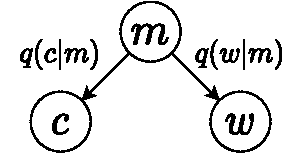
\includegraphics[width=0.49\textwidth]{docs/intro_rate_distortion/graphs/cog_comm_dag.pdf}
    \caption{Illustration of our setting in a DAG.}
    \label{fig:pipeline_dag}
\end{figure}

To better illustrate the problem, we need to start from the directed acyclic graph (DAG) shown in Figure~\ref{fig:pipeline_dag}.
The variables involved in the DAG are listed as follows:

\begin{itemize}[leftmargin=*]
    \item \textbf{meaning $m\in\mathcal{M}$\footnote{In this document, the set of a variable is notated by the corresponding calligraphic capital letter.}}: a meaning $m$ is \textcolor{red}{a discrete variable} indicating the possible meanings.
    It specifies both distributions over $c$, i.e. $q(c|m)$, and distributions over words $w$, i.e. $q(w|m)$.
    In fact, \textcolor{red}{$m$ is the core variable in our project}, and it corresponds to the source variable $x$ in the standard information theory model.
    
    We don't know the size of meaning space $|\mathcal{M}|$ nor $p(m)$ for each $m$.
    In both communication problem and learning problem, we have to infer that out.
    Or, in the language of probabilistic graphical model, $m$ is a latent variable in our setup.
    We will also show in the Section~\ref{sec:comm}and~\ref{sec:learning} that $p(m)$ can be inferred out by algorithms similar to Expectation-Maximisation. 

    \item \textbf{colour chip $c\in\mathcal{C}$}: a colour chip is also a discrete integer variable indicating the possible values of colours. 
    $\mathcal{C}$ is given in the data set, and it keeps identical across different languages (defined below). 
    The colour palette $\mathcal{C}$ we're going to use is shown in Figure~\ref{fig:colour_palette}, where each grid corresponds to a specific $c$.
        \begin{figure}[h]
            \centering
            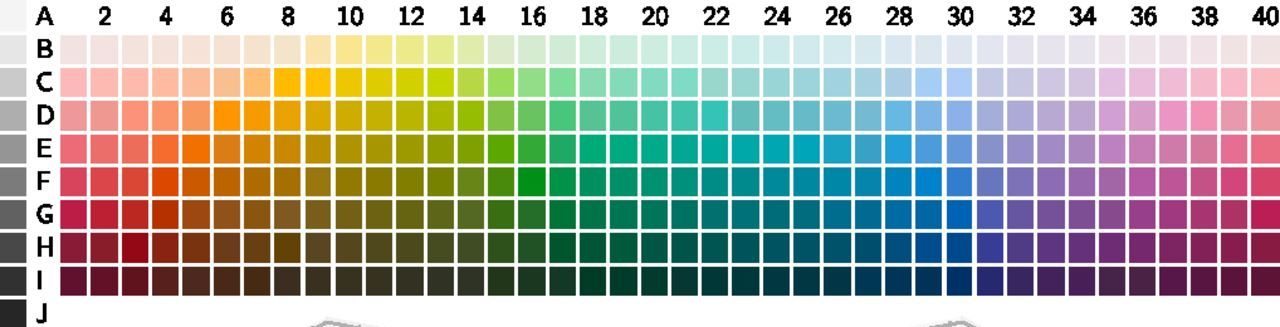
\includegraphics[width=0.49\textwidth]{docs/intro_rate_distortion/graphs/colour_palette.jpg}
            \caption{Colour palette introduced by \citet{berlin1991basic}}
            \label{fig:colour_palette}
        \end{figure}
        
    In this project, we will ignore the variable $u$ (``universe'') used by \citet{zaslavsky2018efficient} because the entire universe is constrained to the colour palette. 
    Mathematically, $\mathcal{U}$ is just a superset of $\mathcal{C}$ which represents the objects in the universe.
    
    Same to \cite{zaslavsky2018efficient}, given a meaning $m$, we assume the conditional distribution of $c$ is a Gaussian centred at $\rc(m)$, i.e.:
    \begin{align}
    q(c|m)\propto \exp{-\frac{1}{\sigma^2}}||c-\rc(m)||^2    
    \end{align}
    
    An example is given in Figure~\ref{fig:green_meaning}.
        \begin{figure}[h]
            \centering
            
\includegraphics[width=0.49\textwidth]{docs/intro_rate_distortion/graphs/green_meaning.png}
            \caption{Meaning of ``green'' which is a Gaussian distribution over different colour chips.}
            \label{fig:green_meaning}
        \end{figure}
        
    \item \textbf{word $w\in\mathcal{W}$}: a discrete variable transmitted from speaker to listener. 
    We can give each value a name, e.g. ``blue'' for the 3rd value.
    However, this is not necessary here since we do not care what actual word is used for some meaning. Sometimes, $\mathcal{W}$ is referred to as ``dictionary'', ``vocabulary'', or ``lexicon''.
    Since the conditional distribution $q(w|c)$ has a name and it's an important concept in this project, so we illustrate it in the following separately.
    
    \item \textbf{language $q(w|m)$}: a language is the distribution of words conditioned on meanings, i.e. a language tells us the probability of emitting a word $w$ given a meaning $m$.
    It is a.k.a. the \emph{encoder} in standard information theory terminology, and can also be written as a function $L:\mathcal{M}\rightarrow\mathcal{W}$.
        \begin{figure}[h]
            \centering
            
\includegraphics[width=0.49\textwidth]{docs/intro_rate_distortion/graphs/color_language.png}
            \caption{English on the colour palette from \citet{berlin1991basic}.
            }
            \label{fig:language_example}
        \end{figure}
    
    An example based on English is illustrated in Figure~\ref{fig:language_example}.
    To be specific, the colour chips in the green region will all be referred by the word ``green''.
    The boundary is hard in this example, but the naming policy $q(w|m)$ can have soft boundaries, e.g. by using Gaussian distribution.
    
    \item \textbf{interpretation policy $q(\hat{m}|w)$\label{par:decoder}}: an interpretation specifies the distribution of colour chips given a specific word, a.k.a. \emph{decoder} in standard information theory terminology, and can also be written as a function $I:\mathcal{W}\rightarrow\mathcal{C}$.
    Note we use $\hat{m}$ here instead of $m$ because the two random variables have different probability mass although they have the same sample space. 
    $\hat{m}$ is the understood or reconstructed meaning from the word $w$.
    For example, after receiving the word ``green'', we could have a distribution over all colours that is very similar to the one in Figure~\ref{fig:green_meaning} but more skewed towards blue.
    
    The $q(\hat{m}|w)$ used by \citet{zaslavsky2018efficient} is a Bayesian learner defined as follow:
    \begin{equation}
        q(\hat{m}|w) \propto q(w|m)p(m)
        \label{eq:bayesian_interpretation}
    \end{equation}
    That is, we can determine $q(\hat{m}|w)$ once we have an established $q(w|m)$ and $p(m)$.
    
    
\end{itemize}

\section{Communication Problem}
\label{sec:comm}

We first illustrate communication problem as all members are more familiar with it and there is no unique variable involved in it.
Our aim in communication part of this project is to give a diagram similar to the one sketched in Figure~\ref{fig:curve_comm}.
The red line in the figure is referred as ``frontier'', and our aim is to show that it is indeed a trade-off curve.
The calculation of each axes and the curve itself are illustrated in the following subsections.

Meanwhile, it is very important to realise that we're going to \textcolor{red}{optimise both $q(w|m)$ and $p(m)$} in the commutation problem to reduce the information loss defined in Section~\ref{ssec:lan_info_loss}.

\begin{figure}[t]
    \centering
    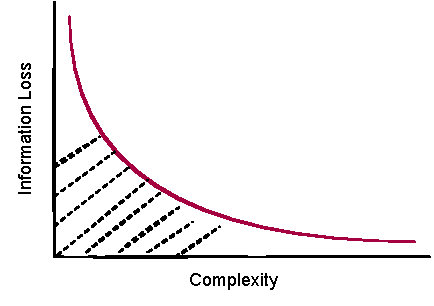
\includegraphics[width=0.49\textwidth]{docs/intro_rate_distortion/graphs/communication_curve.pdf}
    \caption{The curve we aim to plot in the communication problem.}
    \label{fig:curve_comm}
\end{figure}

\subsection{Pipeline}
\label{ssec:pipeline}

The pipeline of our model is shown in Figure~\ref{fig:pipeline}, where $\mathcal{E}$ denotes the error/loss function we're going to use.
Note that there's no $c$ involved in the diagram, since $c$ is not a part of communication but a part of the metric used for evaluating the loss during communication.

\begin{figure}[h]
    \centering
    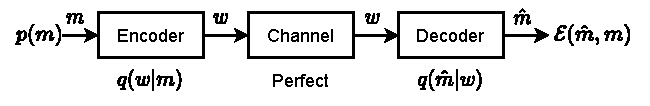
\includegraphics[width=0.49\textwidth]{docs/intro_rate_distortion/graphs/cog_communication.pdf}
    \caption{The pipeline of our model.}
    \label{fig:pipeline}
\end{figure}

In the existing works, the common choices of $\mathcal{E}$ are indicator function $\mathbbm{1}(\hat{m}=m)$ and $KL$-divergence $D[q(c|\hat{m},w)||q(c|m)]$.
since we're going to use $KL$-divergence, the full form of it is given as follow:

\begin{equation}
\begin{split}
    & \mathcal{E}(\hat{m}, m) \triangleq  D[\hat{m}||m] \\
    & = D[q(c|\hat{m},w)||q(c|m)]  \\
    & = \sum_{c} q(c|m) \log \frac{q(c|m)}{q(c|\hat{m},w)} \\
    & = \sum_{c} q(c|m) \log \frac{q(c|m)}{q(c|\hat{m})q(\hat{m}|w)}
\end{split}
\label{eq:comm_loss_function}
\end{equation}

The distortion (a.k.a. information loss with $D[\hat{m}||m]$) is then defined by the expectation of our error/loss function, i.e.

\begin{equation}
    \mathbb{E}_{m,\hat{m}}\left[\mathcal{E}(\hat{m},m)\right]
    \label{eq:distortion}
\end{equation}


\subsection{Complexity of Languages}
\label{ssec:complexity}

The complexity of our a language is defined as the mutual information between $m$ and $w$, i.e. 

\begin{equation}
    I(M;W) = \sum_{m,w} p(m)q(w|m)\log \frac{q(w|m)}{q(w)}
    \label{eq:complexity_definition}
\end{equation}

Given $p(m)$, the amount of information conveyed by it can be measured by the entropy of it, i.e. $H(M)$.
With $H(M)=I(M;W)+H(M|W)$, it is then straightforward to see that $I(M;W)$ is how many extra information about $m$ conveyed by $w$, i.e. the amount of information conveyed in the channel/language.
Assuming that more information means higher complexity, then the complexity of a language can be measured by $I(M;W)$, or at least, there is a positive correlation between the two quantities.

Therefore, once we have a $q(w|m)$, we can calculate its complexity by simply following Equation~\ref{eq:complexity_definition}.
We will show later how to derive such a $q(w|m)$ in Section~\ref{ssec:comm_opt_ib}.

\subsection{Information Loss of Languages}
\label{ssec:lan_info_loss}

As we illustrated in the interpretation policy, given a language and a learner architecture, we can derive $q(\hat{m}|w)$.
Then, the joint distribution of $\hat{m}$ and $m$ is as follow:

\begin{equation}
    \begin{split}
        q(\hat{m},m) 
        & = q(\hat{m}|m)p(m) \\
        & = \sum_w q(\hat{m}|w)q(w|m)p(m)
    \end{split}
    \label{eq:joint_c_hat_c}
\end{equation}

Combining the above equation with Equation~\ref{eq:distortion}, the information loss can then be calculated as:

\begin{equation}
    \begin{split}
        & \mathbb{E}_{q(\hat{m},m)}\left[D[\hat{m}||m]\right] \\
        & = \mathbb{E}_{q(\hat{m},m)}\left[ \sum_{c} q(c|m) \log \frac{q(c|m)}{q(c|\hat{m}, w)} \right] \\
        & = \sum_{\hat{m},m} q(\hat{m}|m)p(m)\sum_{c} q(c|m)\log\frac{q(c|m)}{q(c|\hat{m})q(\hat{m}|w)} \\
        & = \sum_{\hat{m},m,w} q(\hat{m}|w)q(w|m)p(m)\sum_{c} q(c|m)\log\frac{q(c|m)}{q(c|\hat{m})q(\hat{m}|w)} \\
        & = \sum_{\hat{m},m,c,w}q(\hat{m}|w)q(w|m)p(m)q(c|m)\log\frac{q(c|m)}{q(c|\hat{m})q(\hat{m}|w)}
    \end{split}
    \label{eq:comm_info_loss}
\end{equation}

\subsection{Optimising Information Bottleneck}
\label{ssec:comm_opt_ib}

So far, everything seems fine with a given language $q(w|m)$ and a given distribution of meanings $p(m)$.
But, there is still one question: how could we get them?

To do so, we going to optimise the information bottleneck (IB) objective function as follow:



\section{Learning Problem}
\label{sec:learning}

Infer $p(m)$ given $(c,w)$ pairs.

\section{Dataset}
\label{sec:dataset}


\bibliographystyle{acl_natbib}
\bibliography{main}

\end{document}
